\documentclass{article}

\usepackage{epsfig}
\usepackage[export]{adjustbox}% http://ctan.org/pkg/adjustbox
\usepackage{caption}
\usepackage{subcaption}
\usepackage{fullpage}
\usepackage{commath}
\usepackage{amssymb}
\usepackage[space]{grffile}
\usepackage{algorithm, algorithmic}

\def\E{\mathbb{E}}
\def\R{\mathbb{R}}
\def\bin{\text{bin}}
\def\bet{\text{beta}}
\def\range{\text{range}}
\def\vec{\text{vec}}

\newcommand\hide[1]{}

\title{HMM with Contexts in DNA Methylation Problem}

\author{Chicheng Zhang}

\begin{document}
\maketitle


\section{The Model}

We are given sequences $\cbr{m_t, c_t}$, where at each time $t$ the methylation count is $m_t \in \cbr{0,1,\ldots,n}$, and the context information is $c_t \in [c]$. We model the data using a hidden Markov model with context information, that is, the underlying dynamics of the hidden states is driven by a Markov chain $\cbr{y_t}$, where $y_t \in [m]$.

It can be described by parameters $(\pi, T, O)$, where $\pi$ is the initial probability distribution $\Pr(y_1)$ and $T$ is the transition matrix of the Markov chain $\Pr(y_{t+1} | y_t)$, $O$ is the observation matrix, namely the conditional probability of methylation given hidden state and context $\Pr(m_t | c_t, y_t)$. See Figure~\ref{fig:contexthmm} for illustration.

\begin{figure}[h]
\centering
\scalebox{0.3}
{
\includegraphics{hmm.png}
}
\caption{Modeling DNA methylation using a Hidden Markov model with context information.}
\label{fig:contexthmm}
\end{figure}

Our objective is to recover parameters $\pi$, $T$ and $O$ based on iid samples drawn from this model.

\section{Algorithm based on Method of Moments}

For each $i$, consider recovering a block of observation matrix $O^{2, i} = \Pr(m_t | c_t = i, y_t)$ separately. We make the assumption that $O^{2, i}$ is of full column rank. Then, the joint cooccurence tensor of $(m_1, m_2, m_3)$, when the context of observation 2 $c_2$ is $i$, has the following structure:
\[ \E [m_1 \otimes m_2 \otimes m_3 | c_2 = i] = \sum_j \omega_j O^{1}_j \otimes O^{2, i}_j \otimes O^{3}_j \]
where $\omega$ is the distribution of $y_2$ given $c_2$, $O^{1} = \E[m_1 | y_2]$, $O^{2,i} = \E[m_2 | y_2, c_2 = i]$, $O^{3} = \E[m_3 | y_2]$.
At this point, standard tensor decomposition method can readily be applied to extract the columns of $O^{2, i}$.

Alternatively, we have
\[ \E [m_1 \otimes m_3] = \sum_j \omega_j O^1_j \otimes O^3_j \]
and
\[ \E [m_1 \otimes m_2 | c_2 = i] = \sum_j \omega_j O^{1}_j \otimes O^{2, i}_j \]
Then standard symmetrization and orthogonalization routine can be applied to recover the columns of $O^{2, i}$.

\section{Binomial Hidden Markov Model}
In this section, we consider HMMs whose observation matrix has structured columns, that is, columns which are probability mass functions of binomial distribution. We first take a step back, considering HMMs without context information. (The approach can be easily generalized to the setting with context information.)

In this model, each element of $O$ can be written as $O_{i,j} = {n \choose i} p_j^i (1-p_j)^{n-i}$, i.e. the probability that there are $i$ heads out of $n$ trials when flipping a coin with bias $p_j$. Instead of recovering $O$, we now turn to the task of recovering $p_j, j = 1,2,\ldots,m$. A naive approach would be to first recover the columns of $O$, e.g. $O_j$, then get $p_j$ using the formula:

\[ p_j = \sum_{i=0}^n \frac{i}{n} {n \choose i} p_j^i (1-p_j)^{n-i} = \sum_{i=0}^n \frac{i}{n} O_{i,j} \]

\subsection{Exploiting Similarity between Observations}
Sometimes it will be beneficial to consider feature representations of observation other than one-hot encoding. Define feature map $\phi: \cbr{0,\ldots,n} \to \R^D$, where $D$ can potentially be very large, even (uncountably) infinite. For example, $\phi(m) = \cbr{t^m (1-t)^{n-m}}_{t \in [0,1]}$, $\phi(m) = \cbr{t^m (1-t)^{n-m}}_{t \in \cbr{0,0.1, \ldots, 1}}$, or $\phi(m) = \cbr{ \frac{1}{\sqrt{2\pi}} \exp(-(t-m)^2/2)}_{t \in \R}$, etc.

Then, standard method of moments can be applied, resulting in the following representation:
\[ \E [\phi(m_1) \otimes \phi(m_2) \otimes \phi(m_3)] = \sum_j \omega_j O^{1}_j \otimes O^{2}_j \otimes O^{3}_j \]
where $\omega$ is the marginal distribution of $y_2$, $O^{1} = \E[\phi(m_1) | y_2]$, $O^{2} = \E[\phi(m_2) | y_2]$, $O^{3} = \E[\phi(m_3) | y_2]$.

Now, to decompose this $D \times D \times D$ tensor, dimensionality reduction tricks should be applied. After getting an estimate of $O^{2} = \E[\phi(m_2) | y_2]$, we can recover $p_j$'s via algebraic manipulations.


\hide
{
\section{Experiment Results}
\subsection{Setting}
In this set of experiments, we focus on the methylation data in cell type E1 and chromosome 1. At this point we do not take into account the contexts, and we further assume that the coverage in different segments are non-uniform. Let $l$ be the length of the input sequence, $s$ be the number of base segments merged to a single segment, and $n$ be the number of hidden states assumed.

Although the ultimate goal is to recover the transition matrix and observation matrix of the hidden Markov model, at the current stage, we recover $\E[\phi(x, y)|h]$ for each value of $h$. Recall that $x = (c, \mu)$ is the (coverage, methylation) count pair in each segment. The value of $p_h$ for each $h$ can be straightforwardly extracted from $\E[\phi(x, y)|h]$. The transition matrix can also be computed subsequently. We leave the recovery of all the parameters for future work.


%In subsequent results, we show the entire $\E[\phi(x,y)|h]$, as opposed to a single number $p_h \in [0,1]$. The reason is that we wish to recover more information about the hidden states learned, to get a better understanding of the HMM model.

%-- what features $\phi$ are you looking at?
%-- why are you showing the entire $\phi$ vector and not a single number?
We focus on two types of feature mappings $\phi$, the first one is binning mapping:
\[ \phi_{\bin}(x,y) = \begin{cases} {I(\frac{\mu}{c} \in (y,y+h])} & c \neq 0 \\ 0 & c = 0\end{cases} \]
where $h$ is the width of the bins.

The second one is Beta map:
\[ \phi(x,y) = \frac{1}{B(\mu+1, c-\mu+1)}y^\mu (1-y)^{c-\mu} \]
In this mapping there is no explicit notion of ``bin width", but the value of $c$ can be thought of as a parameter controlling it: if the coverage $c$ is large, then the bin width is small, and vice versa.

In experiments, since it is impossible to write down $\E[\phi(x_1, \cdot) \otimes \phi(x_2, \cdot) \otimes \phi(x_3, \cdot)]$ and perform tensor decomposition, we use discretization: compute an empirical version of $\E[\phi(x_1, y_1) \otimes \phi(x_2, y_2) \otimes \phi(x_3, y_3)]$, where $y_1, y_2, y_3$ is in $\cbr{0,h,2h,\ldots,1}$. By decomposing this tensor we are able to recover $\E[\phi(x, y) | h]$, where $y$ is in $\cbr{0,h,2h,\ldots,1}$. By mild regularity assumption on the distribution of $x$, this can give a fairly accurate estimate of $\E[\phi(x, y) | h]$ where $y$ ranges in the $[0,1]$ interval.


\subsection{Effect of Sample Size $l$}
We fix $m = 4$, $s = 1$, and vary the sample size (number of triples collected) $l =$ 1000, 10000, 20000, 40000, 80000, 160000, 320000. The samples are drawn without replacement from the original dataset. Figure~\ref{fig:varyl} shows the result. Note that the value of $m$ is the number of hidden states assumed; for example if $m = 4$, then we get $4$ columns of $\E[\phi(x,y)|h]$. We observe that the output of the algorithm stablizes when $l \geq 80000$.

\begin{figure}[H]

    \begin{tabular}{cc}
    \begin{subfigure}[t]{0.45\textwidth}
        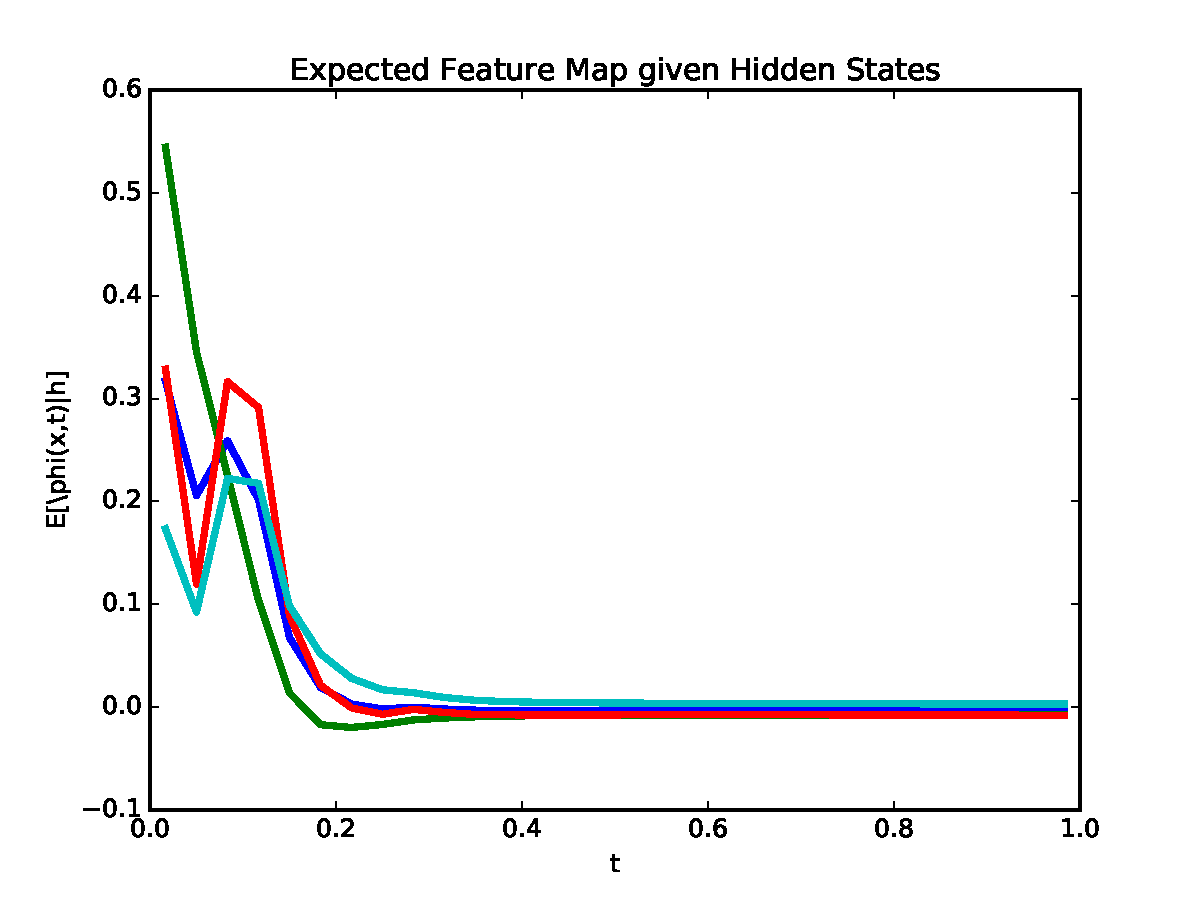
\includegraphics[width=\textwidth]{figs/vary_l/cell = E1_chr = 1_l = 10000_s = 1_m = 4_n = 30_phi = beta_full.pdf}
        \caption{$l = 10000$}
    \end{subfigure}
    &
    \begin{subfigure}[t]{0.45\textwidth}
        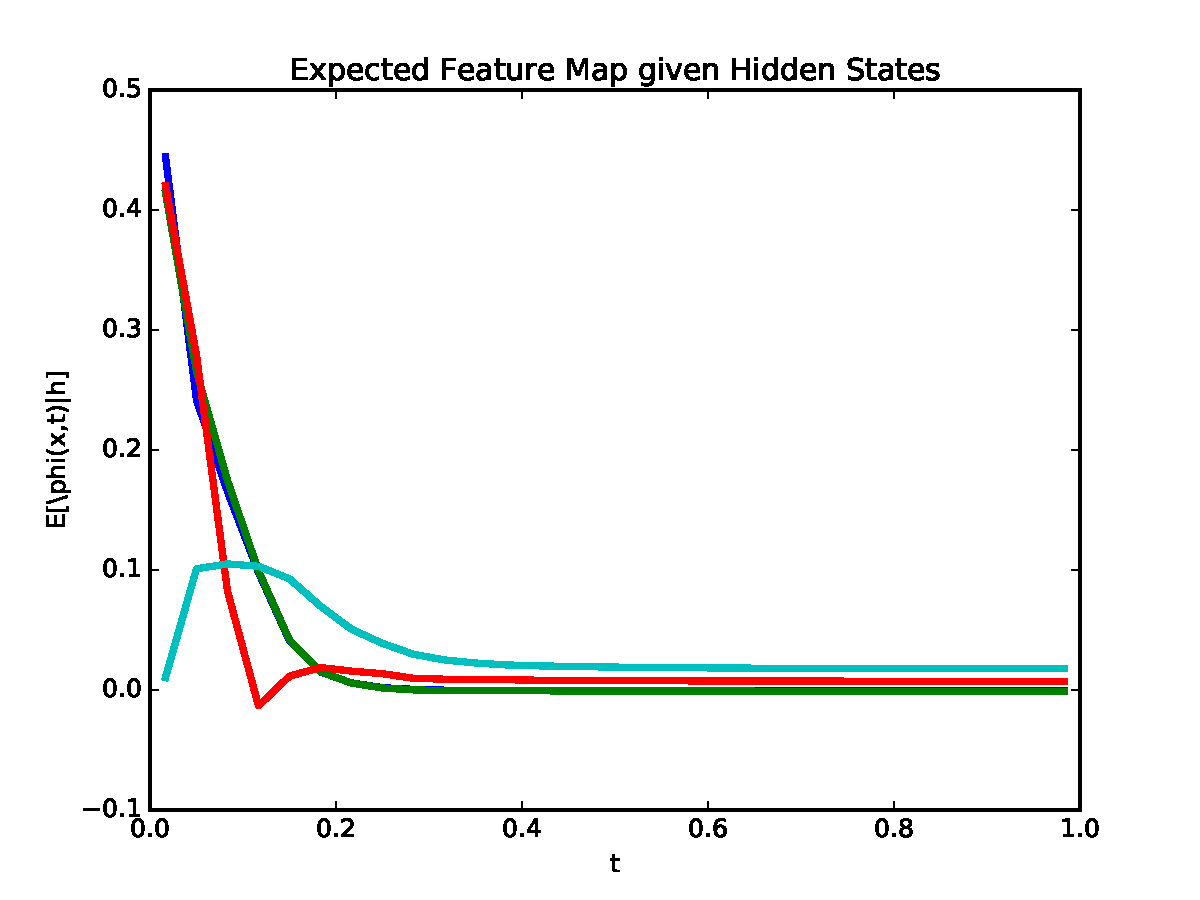
\includegraphics[width=\textwidth]{figs/vary_l/cell = E1_chr = 1_l = 20000_s = 1_m = 4_n = 30_phi = beta_full.pdf}
        \caption{$l = 20000$}
    \end{subfigure}
    \\
    \begin{subfigure}[t]{0.45\textwidth}
        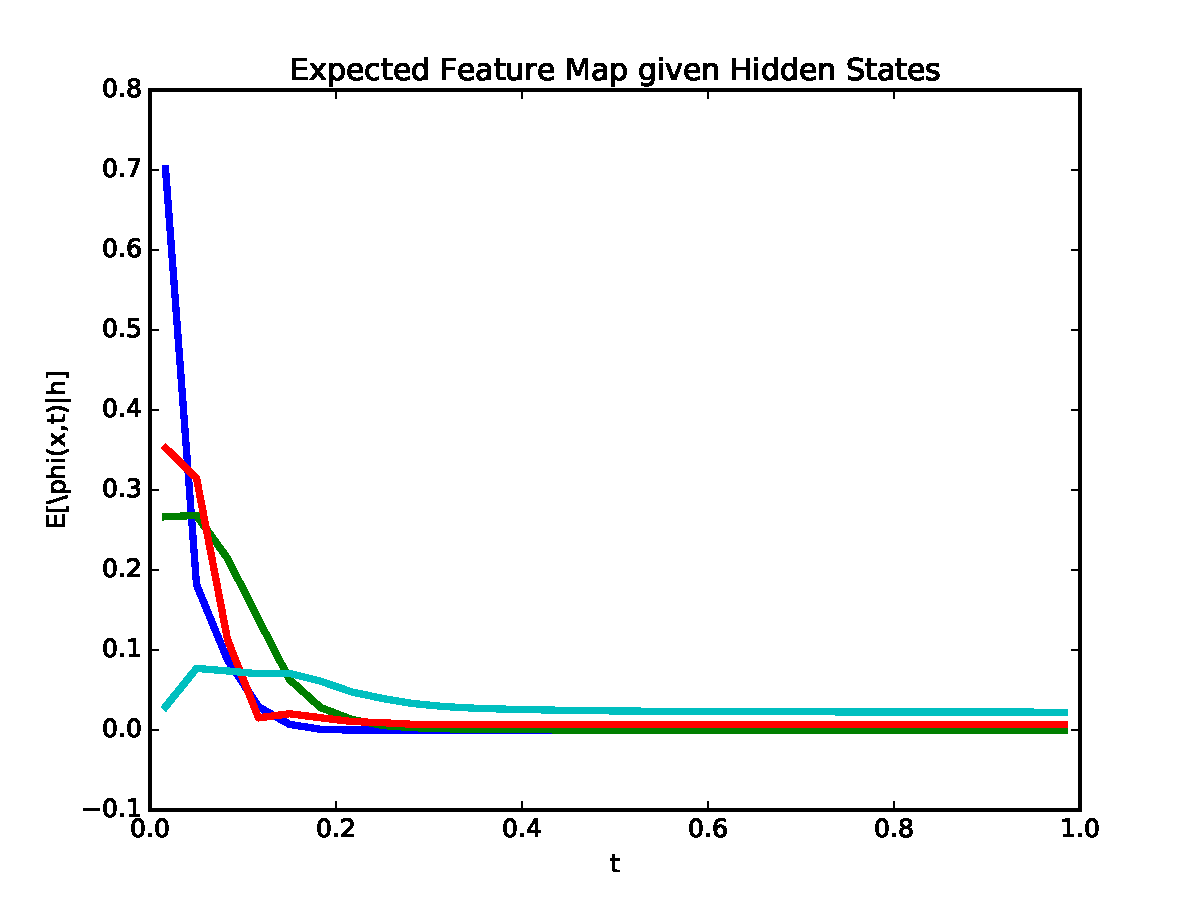
\includegraphics[width=\textwidth]{figs/vary_l/cell = E1_chr = 1_l = 40000_s = 1_m = 4_n = 30_phi = beta_full.pdf}
        \caption{$l = 40000$}
    \end{subfigure}
    &
    \begin{subfigure}[t]{0.45\textwidth}
        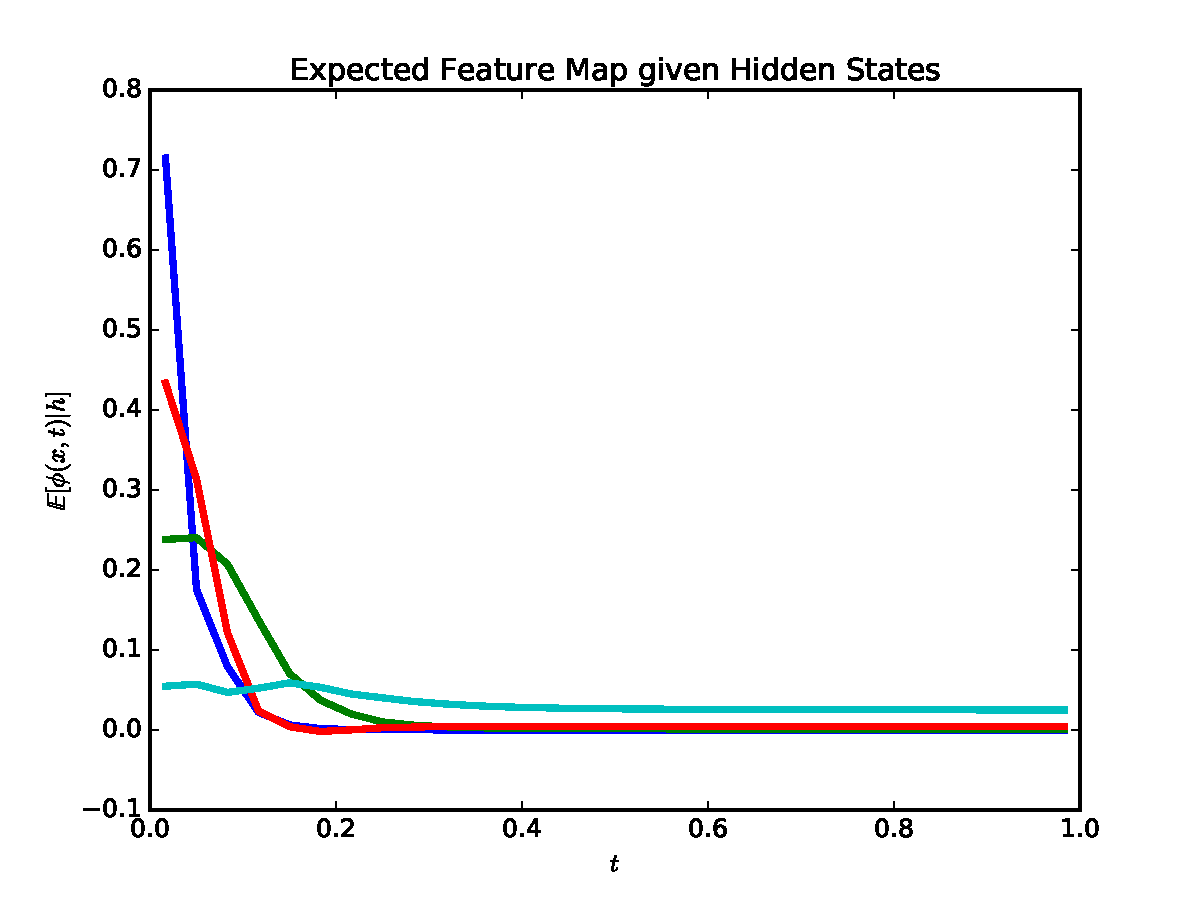
\includegraphics[width=\textwidth]{figs/vary_l/cell = E1_chr = 1_l = 80000_s = 1_m = 4_n = 30_phi = beta_full.pdf}
        \caption{$l = 80000$}
    \end{subfigure}
    \\
    \begin{subfigure}[t]{0.45\textwidth}
        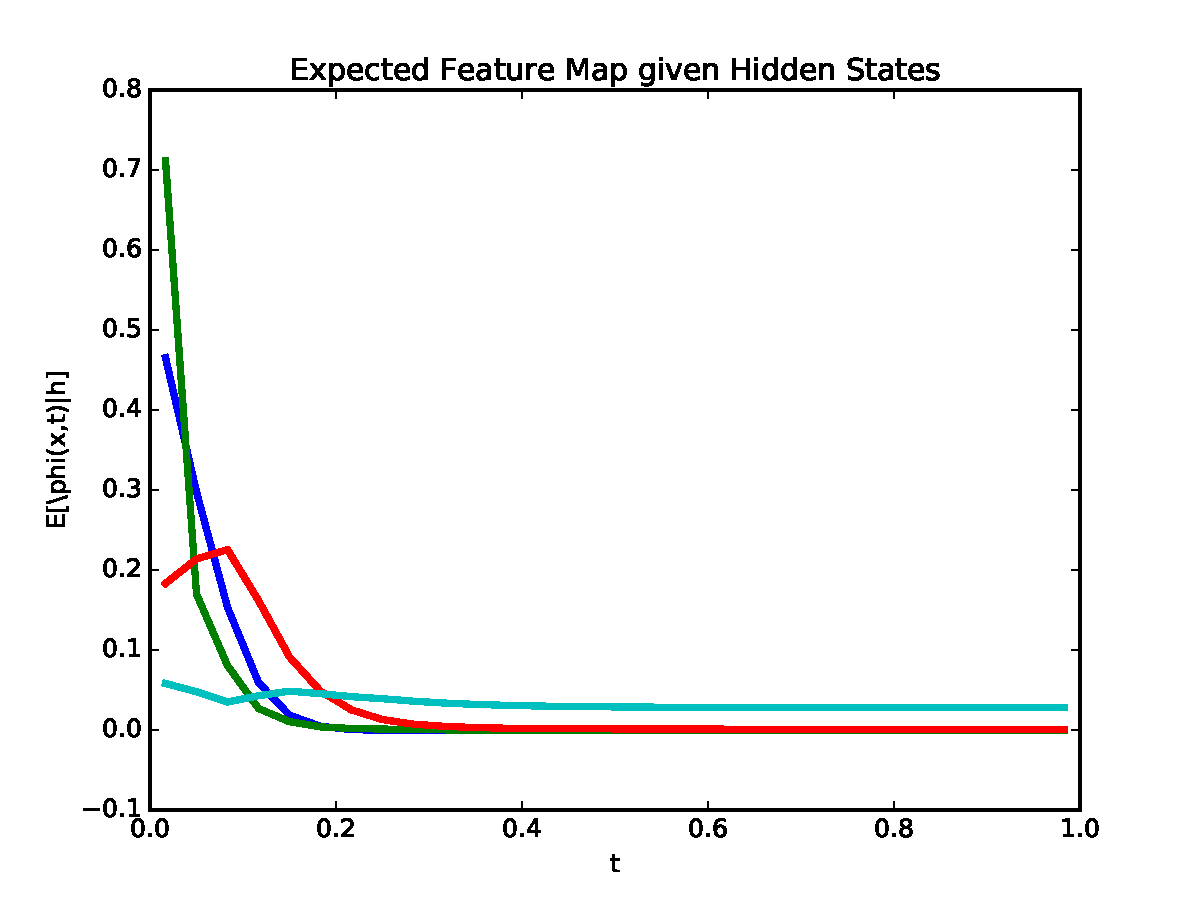
\includegraphics[width=\textwidth]{figs/vary_l/cell = E1_chr = 1_l = 160000_s = 1_m = 4_n = 30_phi = beta_full.pdf}
        \caption{$l = 160000$}
    \end{subfigure}
    &
    \begin{subfigure}[t]{0.45\textwidth}
        \includegraphics[width=\textwidth]{figs/vary_l/cell = E1_chr = 1_l = 320000_s = 1_m = 4_n = 30_phi = beta_full.pdf}
        \caption{$l = 320000$}
    \end{subfigure}
    \\
    \end{tabular}

    \caption{The observation columns recovered $\E[\phi(x,y)|h]$ in terms of $h$, for varying sample size $l$. The $x$-axis is the value of $t$, the $y$-axis is the value of $\E[\phi(x,y)|h]$.}
    \label{fig:varyl}
\end{figure}

\subsection{Effect of Specifying the Number of States}

We fix $l = 320000$, $s = 1$, and vary the number of states $m = 2,3,4,5,6,7,8,9$. Figure~\ref{fig:varym} shows the columns of $\E[\phi(x,y)|h]$ recovered. The spectral algorithm provides reasonable results when $m \leq 4$; when $m \geq 5$, the algorithm started to recover observation columns that has a lot of negative entries.


\begin{figure}[H]

    \begin{tabular}{cc}
    \begin{subfigure}[t]{0.45\textwidth}
        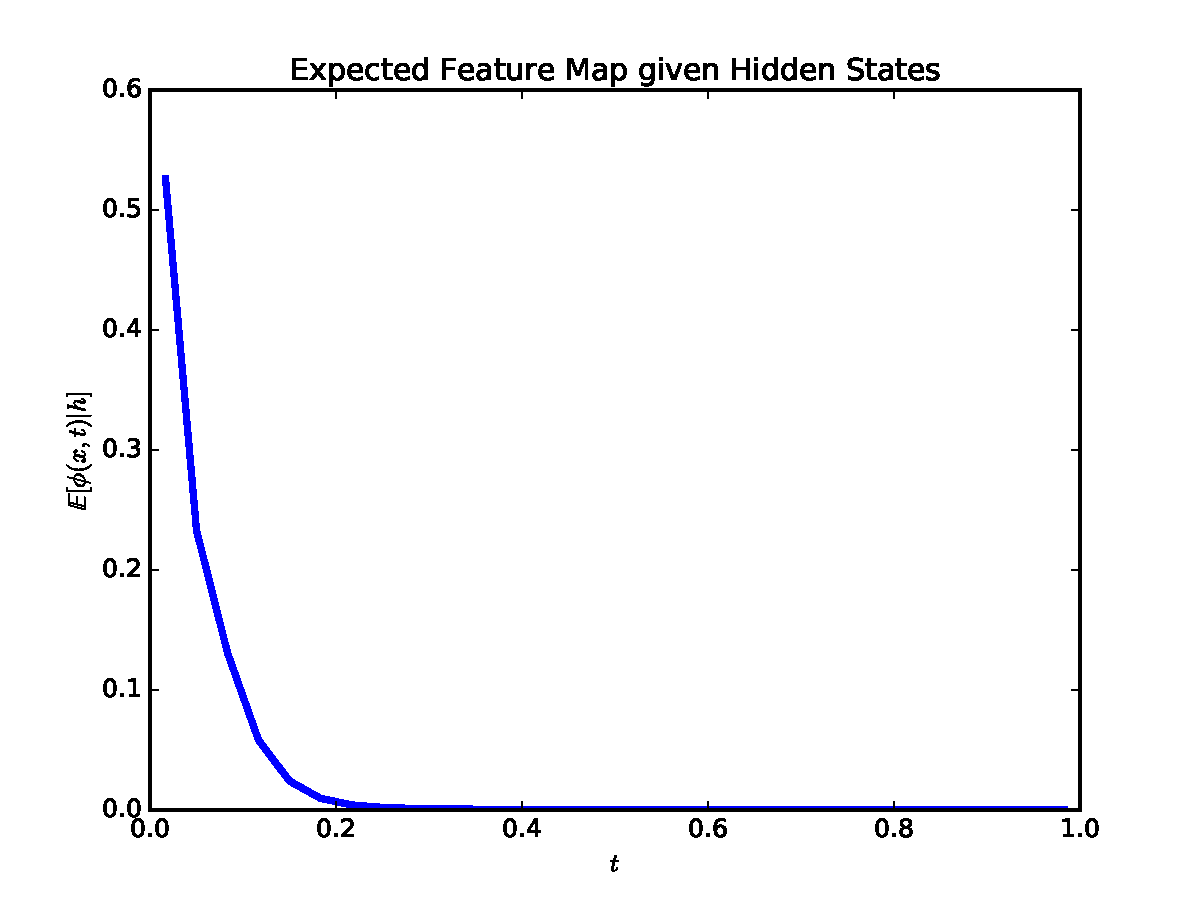
\includegraphics[width=\textwidth]{figs/vary_l/cell = E1_chr = 1_l = 320000_s = 1_m = 1_n = 30_phi = beta_full.pdf}
        \caption{$m = 1$}
    \end{subfigure}
    &
    \begin{subfigure}[t]{0.45\textwidth}
        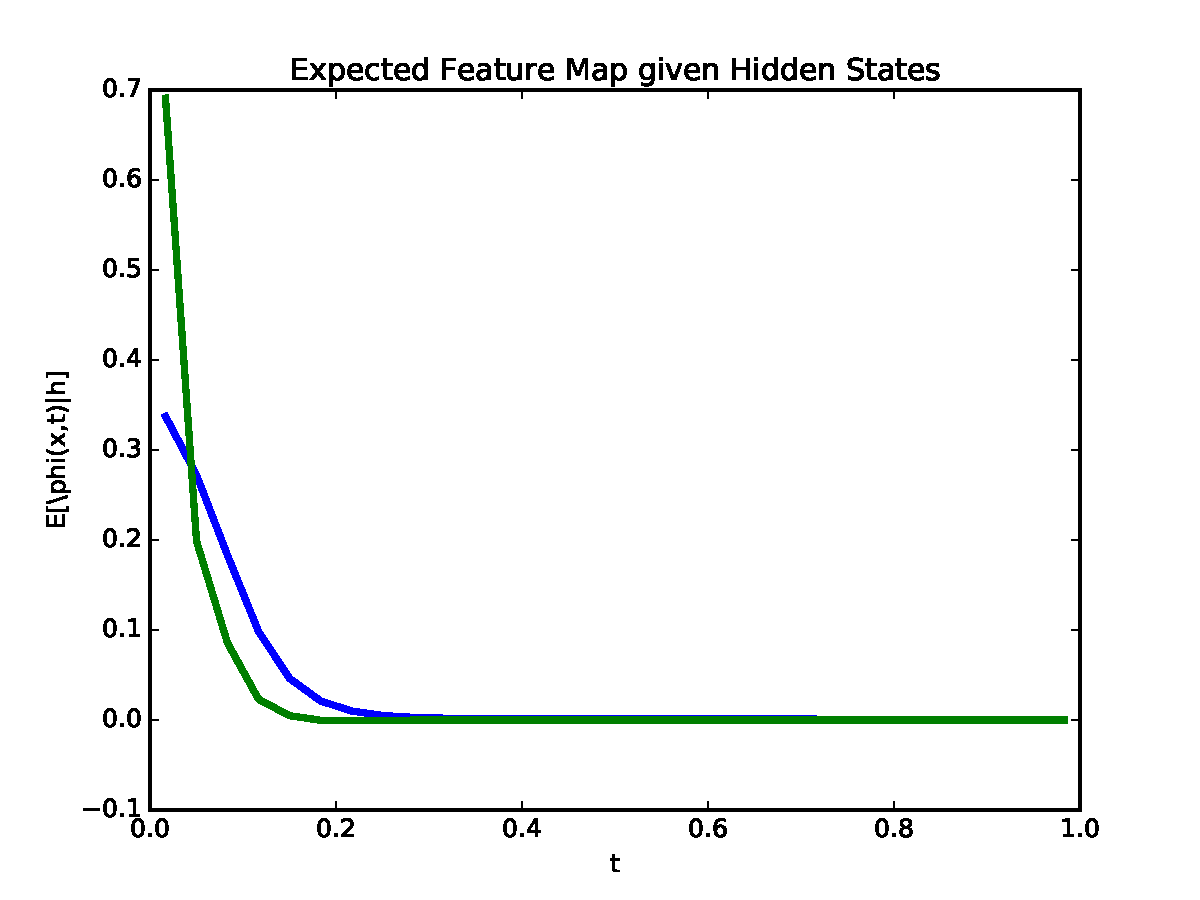
\includegraphics[width=\textwidth]{figs/vary_l/cell = E1_chr = 1_l = 320000_s = 1_m = 2_n = 30_phi = beta_full.pdf}
        \caption{$m = 2$}
    \end{subfigure}
    \\
    \begin{subfigure}[t]{0.45\textwidth}
        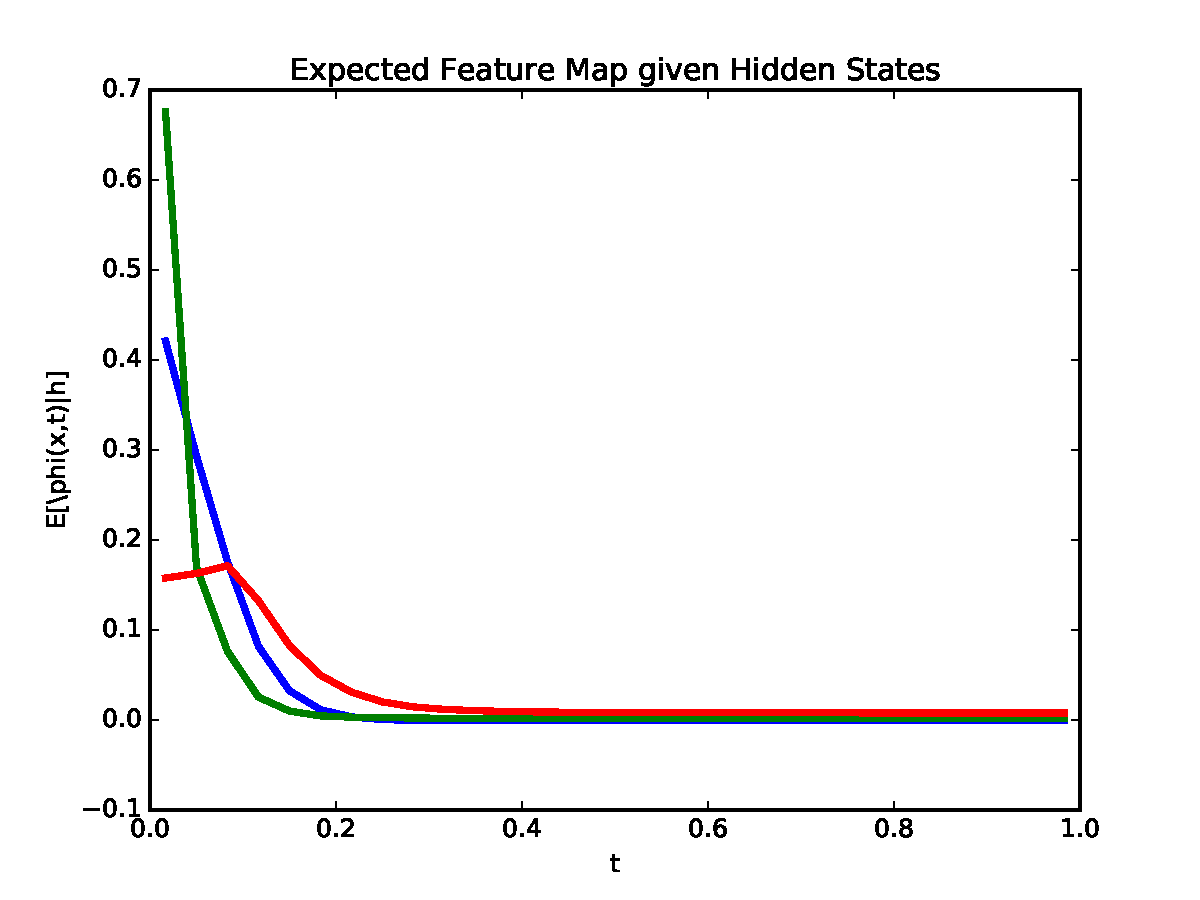
\includegraphics[width=\textwidth]{figs/vary_l/cell = E1_chr = 1_l = 320000_s = 1_m = 3_n = 30_phi = beta_full.pdf}
        \caption{$m = 3$}
    \end{subfigure}
    &
    \begin{subfigure}[t]{0.45\textwidth}
        \includegraphics[width=\textwidth]{figs/vary_l/cell = E1_chr = 1_l = 320000_s = 1_m = 4_n = 30_phi = beta_full.pdf}
        \caption{$m = 4$}
    \end{subfigure}
    \\
    \begin{subfigure}[t]{0.45\textwidth}
        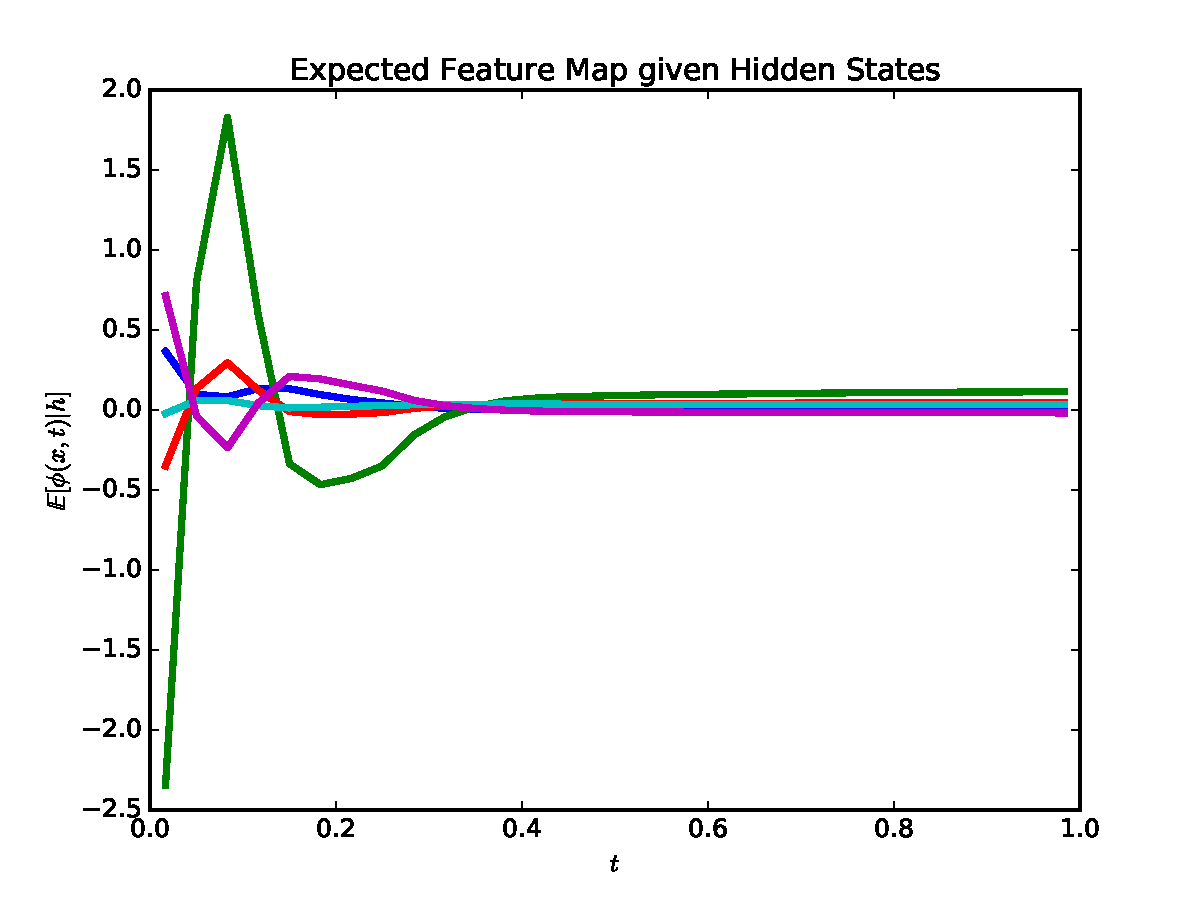
\includegraphics[width=\textwidth]{figs/vary_l/cell = E1_chr = 1_l = 320000_s = 1_m = 5_n = 30_phi = beta_full.pdf}
        \caption{$m = 5$}
    \end{subfigure}
    \end{tabular}

    \caption{The observation columns recovered $\E[\phi(x,y)|h]$ in terms of $h$, for varying number of states $m$. The $x$-axis is the value of $t$, the $y$-axis is the value of $\E[\phi(x,y)|h]$.}
    \label{fig:varym}
\end{figure}

\subsection{Binning Feature vs. Beta Feature}

We compare the experimental results using two types of feature maps $\phi_{\bin}$ and $\phi_{\bet}$. Although the two mappings are substantially different, their respective $\E[\phi(x,y)|h]$ have some similarities. In some sense, the beta mapping is performing a ``soft'' binning which takes into account the number count $c$ in $x$: fixing the value of methylation probability $m/c$, if $c$ is larger, then the beta mapping is closer to a binning mapping with smaller bin size. Figure~\ref{fig:varyphi} shows the columns of the resulting $\E[\phi(x,y)|h]$ recovered. Generally, $\phi_{\bet}$ produces smoother observation columns.

%-- double check this one experiment -- typo in file naming?

\begin{figure}[H]
    \begin{tabular}{cc}
        \begin{subfigure}[t]{0.45\textwidth}
        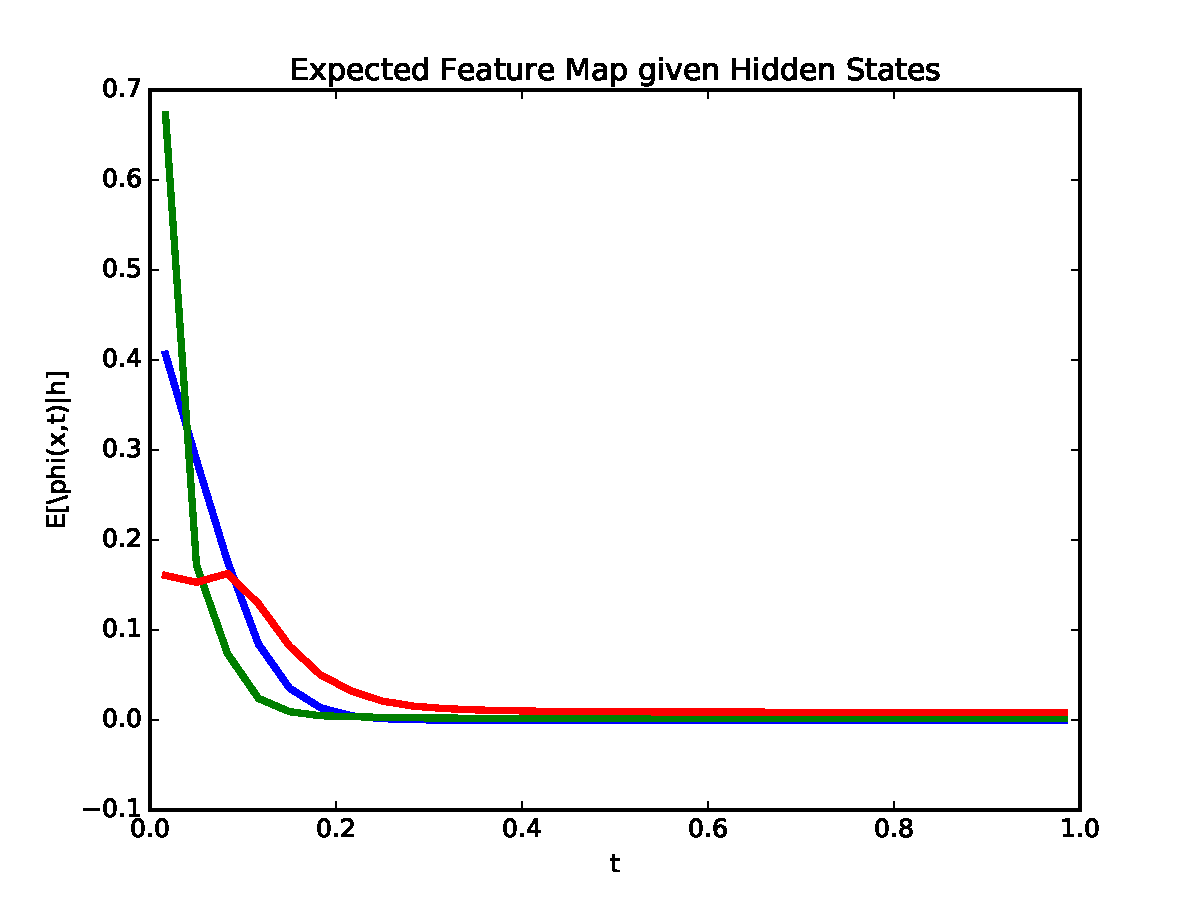
\includegraphics[width=\textwidth]{figs/vary_phi/cell = E2_chr = 1_l = 320000_s = 1_m = 3_n = 30_phi = beta_full.pdf}
        \caption{$\phi = \phi_{\bet}$ is beta mapping, $m = 3$}
    \end{subfigure}
    &
    \begin{subfigure}[t]{0.45\textwidth}
        \includegraphics[width=\textwidth]{figs/vary_phi/cell = E2_chr = 1_l = 320000_s = 1_m = 3_n = 30_phi = binning_igz.pdf}
        \caption{$\phi = \phi_{\bin}$ is binning mapping, $m = 3$}
    \end{subfigure}
    \\
    \begin{subfigure}[t]{0.45\textwidth}
        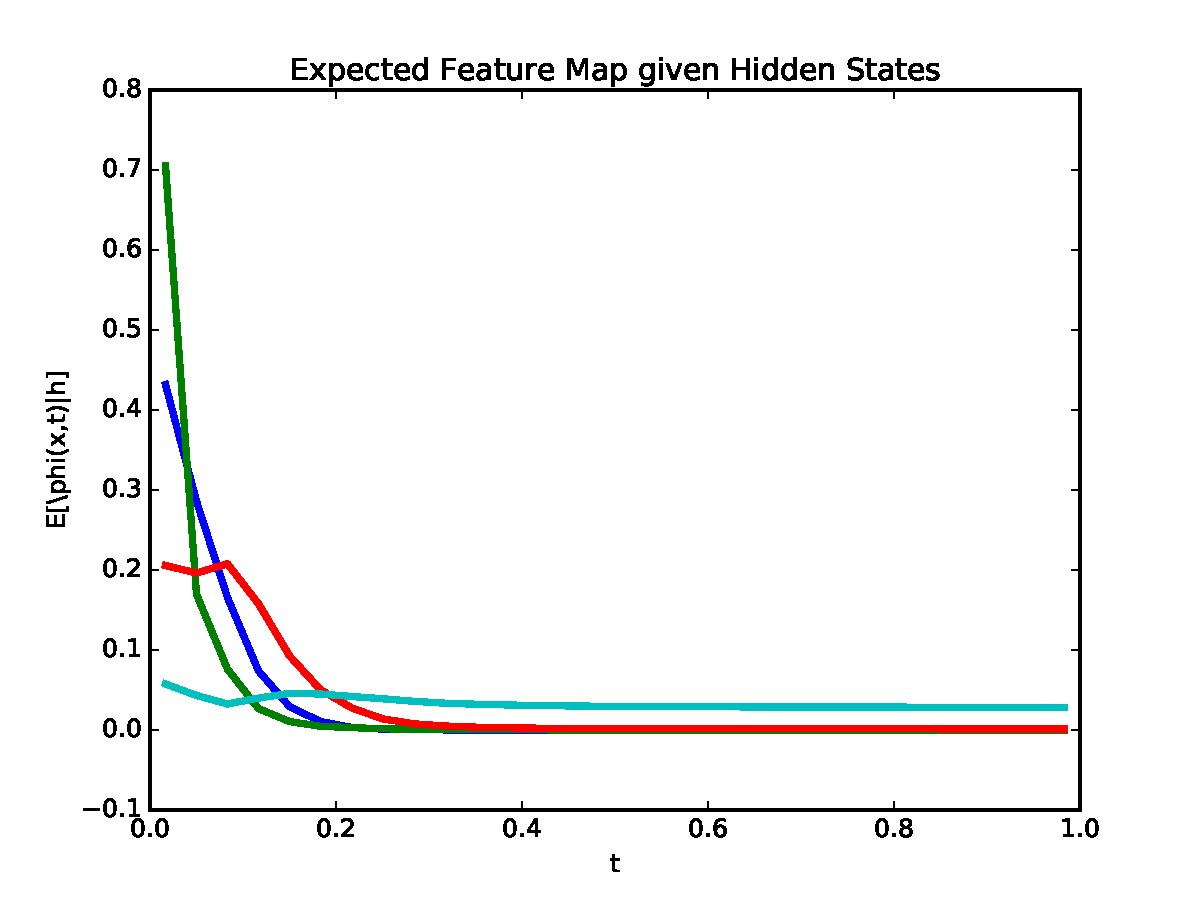
\includegraphics[width=\textwidth]{figs/vary_phi/cell = E2_chr = 1_l = 320000_s = 1_m = 4_n = 30_phi = beta_full.pdf}
        \caption{$\phi = \phi_{\bet}$ is beta mapping, $m = 4$}
    \end{subfigure}
    &
    \begin{subfigure}[t]{0.45\textwidth}
        \includegraphics[width=\textwidth]{figs/vary_phi/cell = E2_chr = 1_l = 320000_s = 1_m = 4_n = 30_phi = binning_igz.pdf}
        \caption{$\phi = \phi_{\bin}$ is binning mapping, $m = 4$}
    \end{subfigure}
    \end{tabular}

    \caption{The observation columns recovered $\E[\phi(x,y)|h]$ in terms of $h$, for $m = 4$ and two types of feature map $\phi$. The $x$-axis is the value of $t$, the $y$-axis is the value of $\E[\phi(x,y)|h]$.}
    \label{fig:varyphi}
\end{figure}

\subsection{Effect of Number of Segments Combined}
We fix $l = 320000$, $m = 4$, and vary the number of merged segments $s = 1,2,3,4,5,6,7,8$. Figure~\ref{fig:varys} shows the columns of the resulting $\E[\phi(x,y)|h]$. It can be seen that the recovered result is fairly insensitive to the choice of $s$.

\begin{figure}[H]
    \begin{tabular}{cc}
    \begin{subfigure}[t]{0.45\textwidth}
        \includegraphics[width=\textwidth]{figs/vary_s/cell = E1_chr = 1_l = 320000_s = 1_m = 4_n = 30_phi = beta_full.pdf}
        \caption{$s = 1$}
    \end{subfigure}
    &
    \begin{subfigure}[t]{0.45\textwidth}
        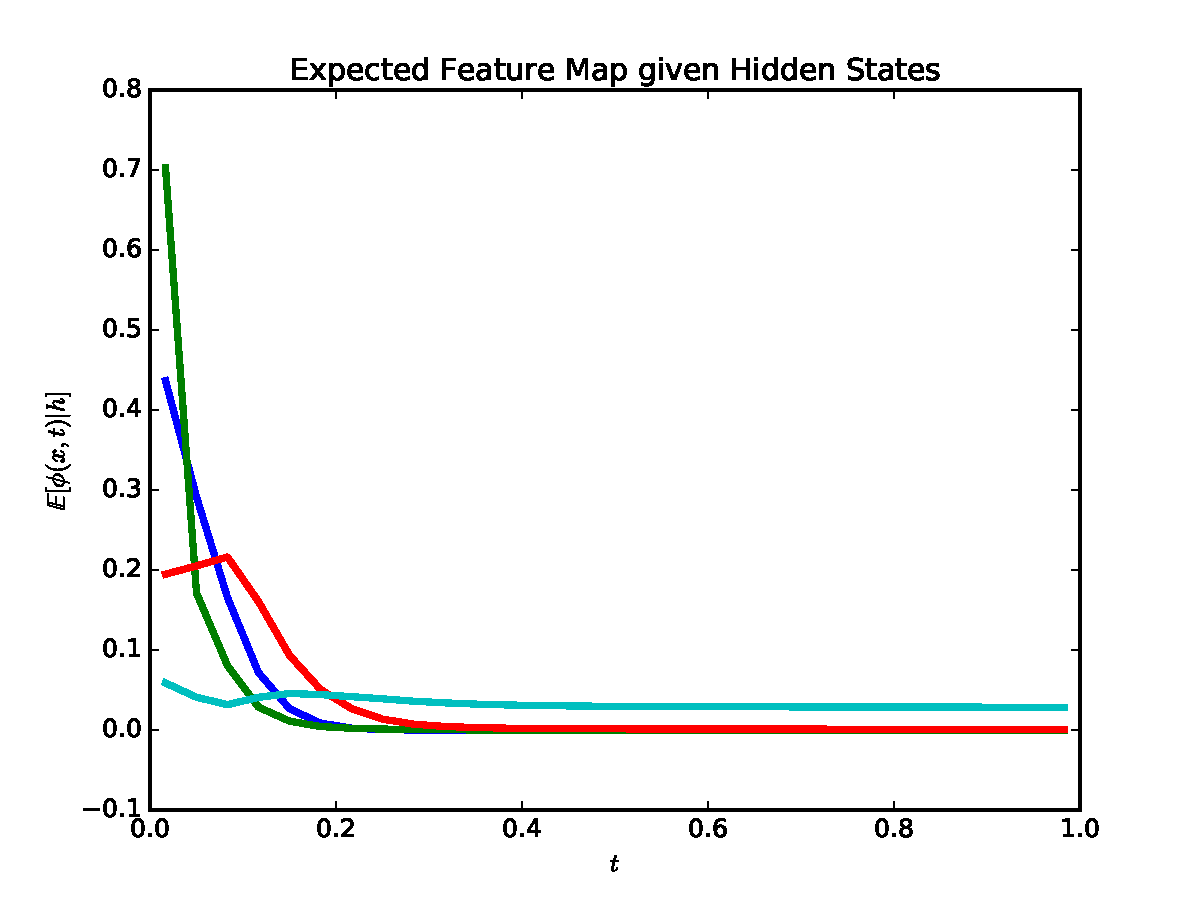
\includegraphics[width=\textwidth]{figs/vary_s/cell = E1_chr = 1_l = 320000_s = 2_m = 4_n = 30_phi = beta_full.pdf}
        \caption{$s = 2$}
    \end{subfigure}
    \\
    \begin{subfigure}[t]{0.45\textwidth}
        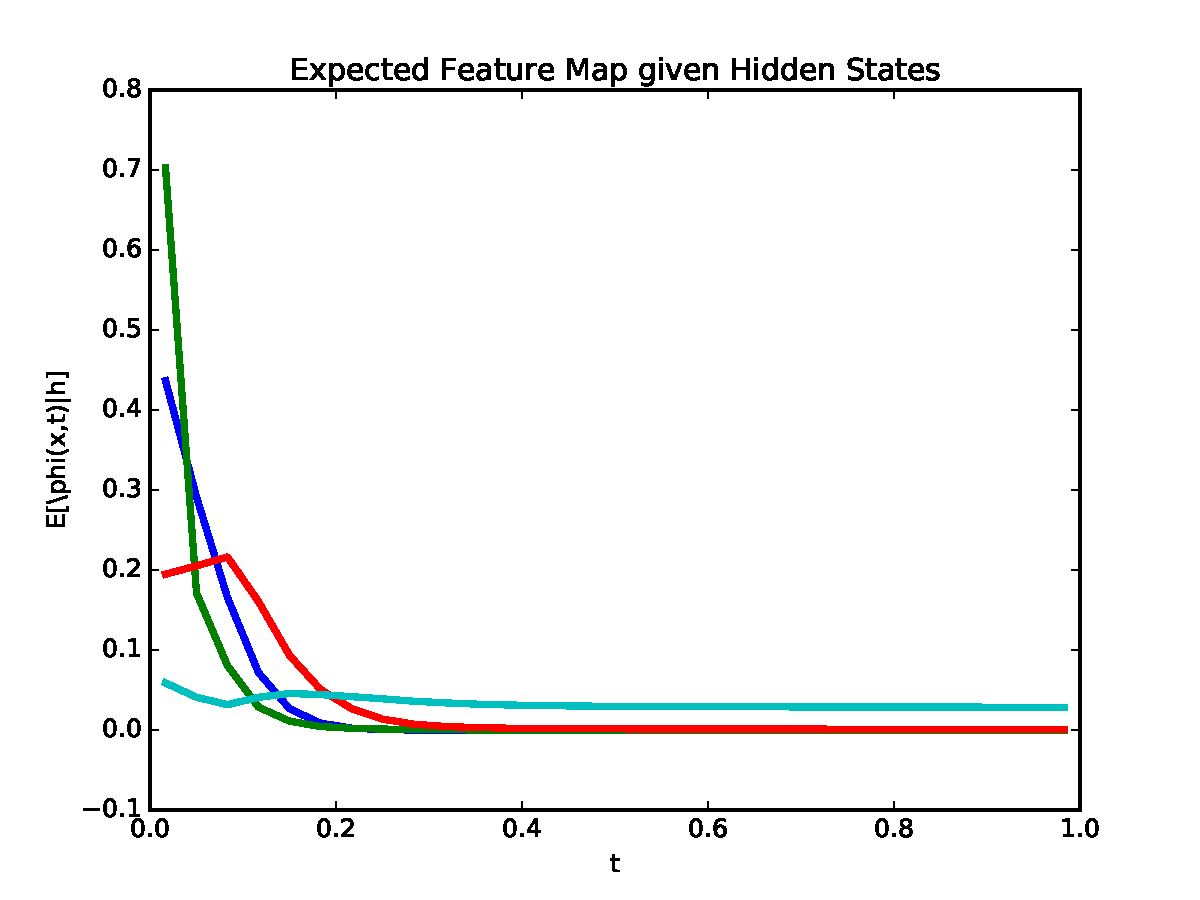
\includegraphics[width=\textwidth]{figs/vary_s/cell = E1_chr = 1_l = 320000_s = 3_m = 4_n = 30_phi = beta_full.pdf}
        \caption{$s = 3$}
    \end{subfigure}
    &
    \begin{subfigure}[t]{0.45\textwidth}
        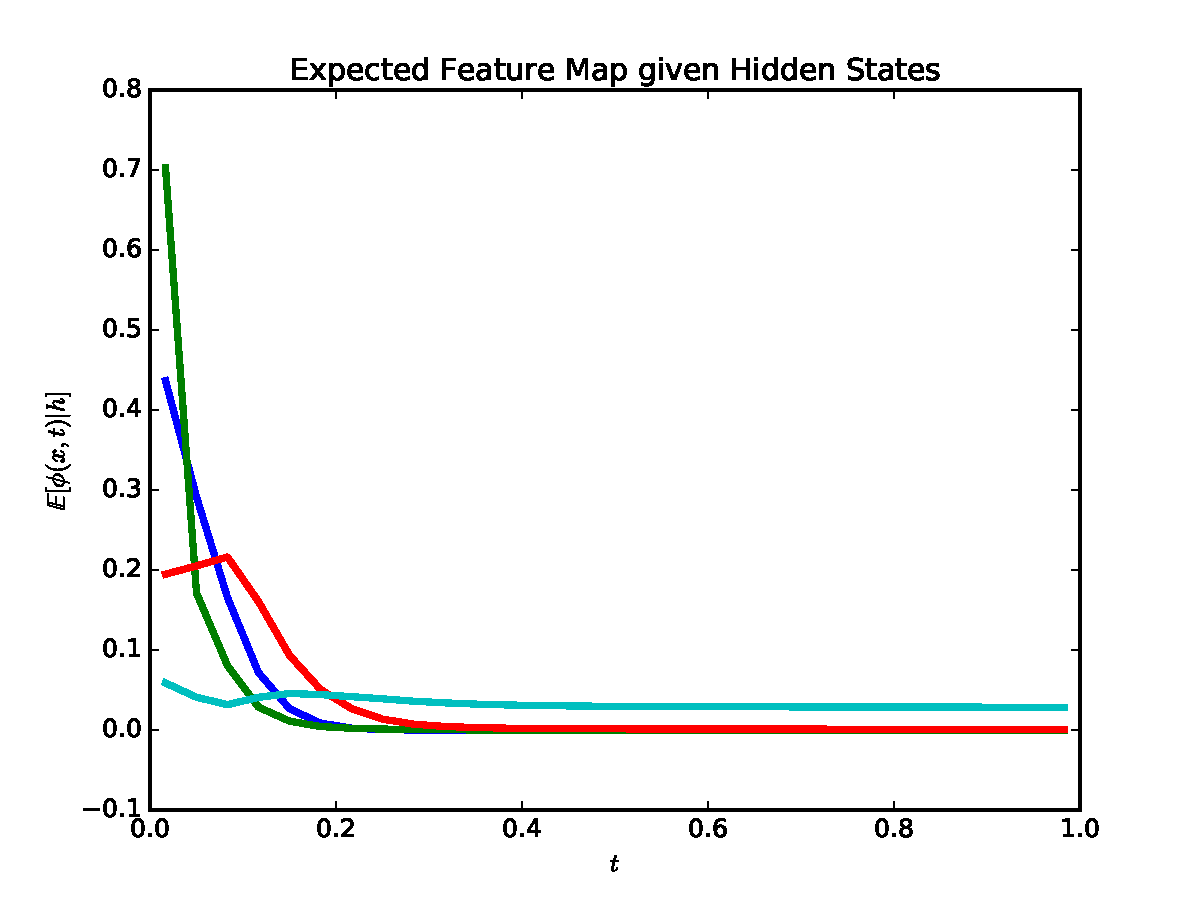
\includegraphics[width=\textwidth]{figs/vary_s/cell = E1_chr = 1_l = 320000_s = 4_m = 4_n = 30_phi = beta_full.pdf}
        \caption{$s = 4$}
    \end{subfigure}
    \\
    \begin{subfigure}[t]{0.45\textwidth}
        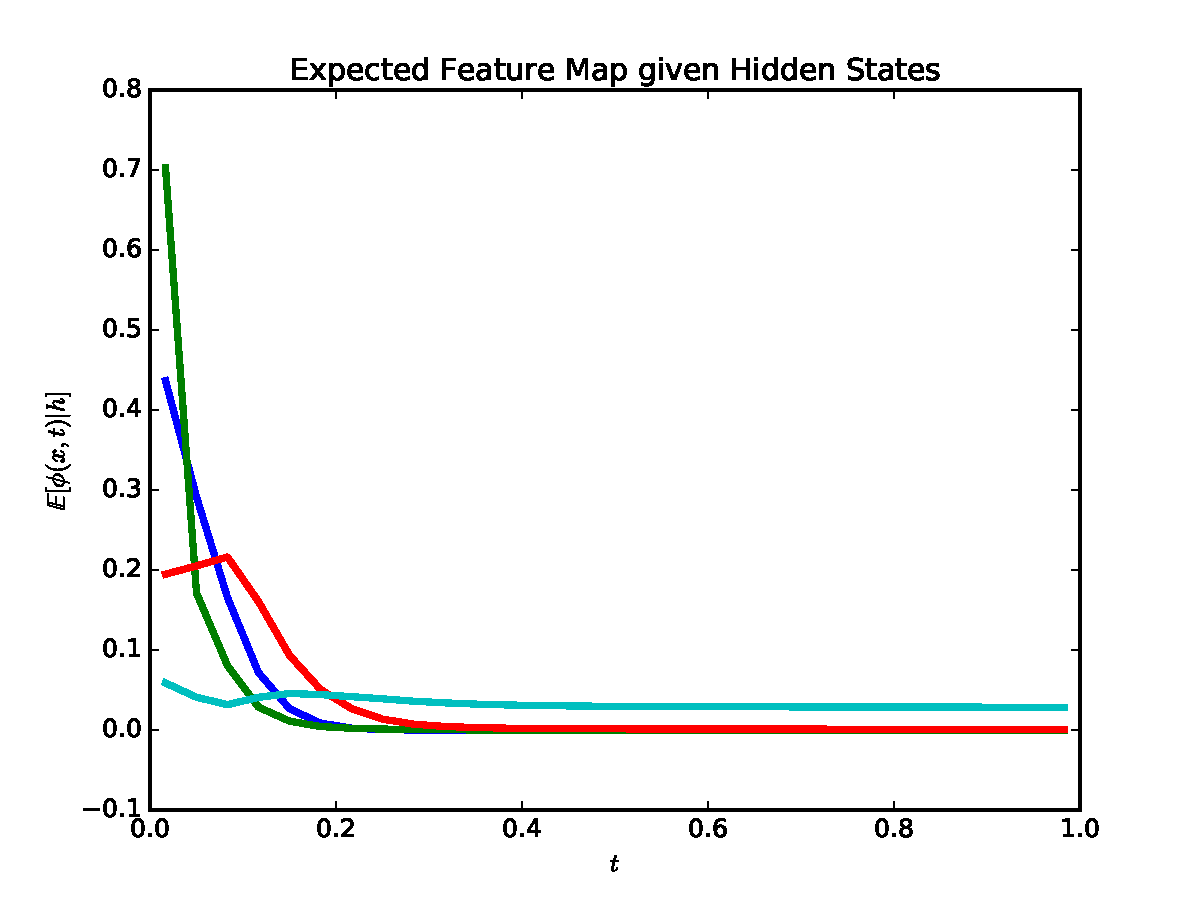
\includegraphics[width=\textwidth]{figs/vary_s/cell = E1_chr = 1_l = 320000_s = 5_m = 4_n = 30_phi = beta_full.pdf}
        \caption{$s = 5$}
    \end{subfigure}
    \end{tabular}

    \caption{The observation columns recovered $\E[\phi(x,y)|h]$ in terms of $h$, for $m = 4$ and two types of feature map $\phi$. The $x$-axis is the value of $t$, the $y$-axis is the value of $\E[\phi(x,y)|h]$.}
    \label{fig:varys}
\end{figure}
}

\section{Possible Variants of Model}

\begin{figure}
  \caption{Possible Variants of the Model}
  \centering
  \includegraphics[width=0.8\textwidth]{model_doubt.jpg}
  \label{fig:modeldoubt}
\end{figure}

In the data given, we are not able to observe the context information on exact positions.
Instead, the data is grouped every 100 base pairs, where in each group, we observe
32 numbers $\cbr{(m_{t,i}, c_{t,i})}_{i=1}^{16}$, two for each context, representing
total coverage and total methylation in context-location specific manner.

We can model the data in the following two graphical models (see Figure~\ref{fig:modeldoubt}). The first one models
the sequence in each context separately. The hidden states are not only context specific,
but also location specific. It is not clear -- at least at this moment -- if we should
align the hidden states across different contexts.

The second model is to put the hidden state as the shared information across different
contexts. Then it assumes that given the hidden states, the 16 observations are conditionally
independent. We suspect this is too strong, and it might be preferable to assume the
16 observations to have dependency and directly build a wholistic feature map based
on them altogether.

\section{Efficient Joint Parameter Estimation of Multiple HMMs}
In this section we study the following probem.
Suppose we are given sequences drawn from two HMMs, and we have the prior knowledge that
the parameters of the two HMMs are close to each other.
Furthermore, suppose we have computed the moments from training data
(denoted as $P_{ij}, \tilde P_{ij}$, $P_{ijk}, \tilde P_{ijk}$ for all $(i,j,k)$ pairs).
The goal is to perform method of moments estimating the parameters of the two HMMs.

It is known that
\[ P_{i,j} = \E[x_i \otimes x_j] = \sum_{l=1}^m w_l (O_i)_l \otimes (O_j)_l \]
and
\[ P_{i,j,k} = \E[x_i \otimes x_j \otimes x_k] = \sum_{l=1}^m (O_i)_l \otimes (O_j)_l \otimes (O_k)_l \]

\subsection{Algorithmic Primitive}
\paragraph{Matrix Regularized Least Squares} In subsequent discussions, the following optimization problem is often considered:
\[ \min_{B \in \R^{n \times k}} f(B) = \| M - A B^T \|_F^2 + \lambda \| B - \tilde{B} \|_F^2 \]
where $M \in \R^{m \times n}$, $A \in \R^{m \times k}$ are given.

This optimization problem an be solved by noticing it can be decomposed to functions with
respect to rows of $B$, that is, $B^{1}, \ldots, B^{m}$.
This gives rise to the following optimization problem:
\[ \min_{B^i \in \R^k} \| M_i - A (B^i)^T \|^2 + \lambda \| B^i - \tilde B^i \|^2 \]
Taking derivatives, we have
\[ 2 A^T A (B^i)^T - 2 A^T M_i + 2 \lambda ((B^i)^T - (\tilde B^i)^T) = 0 \]
that is,
\[ (B^i)^T = (\lambda I + A^T A)^{-1} (A^T M_i + \lambda (\tilde B^i)^T ) \]
horizonally stacking the solution, we get
\[ B^T = (\lambda I + A^T A)^{-1} (A^T M + \lambda \tilde B^T) \]
that is, $B = (M^T A + \lambda B)(\lambda I + A^T A)^{-1}$.
(As a sanity check, when $\lambda = 0$, $B = (A^+ M)^T$, which is the correct solution.)

\paragraph{Weighted Extensions} It is sometimes desirable to consider the following
optimization objective:
\[ \min_{B \in \R^{n \times k}} f(B) = \| M - A B^T \|_F^2 + \lambda \| C (B - \tilde{B}) \|_F^2 \]
where $C \in \R^{p \times n}$ is a linear transformation (the objective aims to measure the
$\ell_2$ similarity of transformed $B$.)
Unfortunately, the solution does not admit a succinct representation. But we can still
write the solution. First, let $\vec(B) = ((B^1)^T, (B^2)^T, \ldots, (B^n)^T)$.
We rewrite the objective as:
\[ f(B) = \sum_{i=1}^n \| M_i - A (B^i)^T \|_2^2 + \sum_{j=1}^k \| C B_j - C B_j \|_2^2 \]
Thus, we can formulate the problem as the following least squares problem:
\[
   \begin{bmatrix} M_{11} \\ \ldots \\ M_{m1} \\ \ldots \\ M_{1n} \\ \ldots \\ M_{mn} \\ C^1 \tilde B_1 \\ \ldots \\ C^{n'} \tilde B_1 \\ \ldots \\ C^1 \tilde B_k \\ \ldots \\ C^{n'} \tilde B_k \end{bmatrix}
   =
   \begin{bmatrix}
     & A^1 & \\ & \ldots & \\ & A^m & \\  & & & \ldots & & & \\ & & & & & A^1 \\ & & & & & \ldots \\ & & & & & A^m \\
     C_{1,1} & & \ldots & & C_{1,n} \\& & \ldots \\ C_{n',1} & & \ldots & & C_{n',n} \\ & & \ldots \\
      & & C_{1,1}  &  & \ldots & & C_{1,n} \\& & & & \ldots \\  & & C_{n',1}  &  & \ldots & & C_{n',n}
   \end{bmatrix} \cdot \vec(B)
\]
Letting the vector in the left hand side as $Y$ and the matrix on the right hand side as $H$, we get $\vec(B) = H^+ Y$.

\paragraph{Basic Weighted Least Squares}
Suppose we would like to solve the following least squares problem:
\[ \min f(\tau) = \| T - \sum_{i=1}^k \tau_i T_i \|_F^2 \]
This is equivalent to solving the following equation:
\[
  \begin{bmatrix} T \cdot T_1 \\ \ldots \\ T \cdot T_k \end{bmatrix}
  =
  \begin{bmatrix} T_1 \cdot T_1 & \ldots & T_1 \cdot T_k \\ \ldots & \ldots & \ldots \\ T_k \cdot T_1 & \ldots & T_k \cdot T_k \end{bmatrix} \cdot \tau
\]
Specifically, if $T_i = a_i \cdot b_i \cdot c_i$, then the equation becomes
\[
  \begin{bmatrix} T(a_1, b_1, c_1) \\ \ldots \\ T(a_k, b_k, c_k) \end{bmatrix}
  =
  \begin{bmatrix} (a_1 \cdot a_1) (b_1 \cdot b_1) (c_1 \cdot c_1) & \ldots & (a_1 \cdot a_k) (b_1 \cdot b_k) (c_1 \cdot c_k) \\ \ldots & \ldots & \ldots \\ (a_k \cdot a_1) (b_k \cdot b_1) (c_k \cdot c_1) & \ldots & (a_k \cdot a_k) (b_k \cdot b_k) (c_k \cdot c_k) \end{bmatrix} \cdot \tau
\]
that is,
\[ \tau = ((A^T A) \circ (B^T B) \circ (C^T C))^{-1}  \begin{bmatrix} T(a_1, b_1, c_1) \\ \ldots \\ T(a_k, b_k, c_k) \end{bmatrix} \]


\subsection{Basic Algorithm}
Define tensor $T = P_{123}(U_1,U_2,U_3) = \sum_i w_i (U_1^TO_1)_i \otimes (U_2^TO_2)_i \otimes (U_3^TO_3)_i$

Given rank parameter $m$, we define objective function $F$ as follows:
\[ F(\tau, A, B, C, \tilde\tau, \tilde A, \tilde B, \tilde C) = \| \sum_{i=1}^m \tau_i A_i \otimes B_i \otimes C_i - T \|_F^2 + \| \sum_{i=1}^m \tilde\tau_i \tilde A_i \otimes \tilde B_i \otimes \tilde C_i - \tilde T \|_F^2 + \lambda \| B - \tilde B \|_F^2 \]

We have the following alternating minimization algorithm for the objective function.

\begin{algorithm}
  \caption{Efficient Joint Parameter Estimation; Basic Algorithm}
\begin{algorithmic}[H]
\STATE Randomly initialize $A, B, C, \tau, \tilde A, \tilde B, \tilde C, \tilde \tau$.
\FOR{$t=1,2,\ldots$:}
\STATE Update $A$: $A \gets \del{\del{\lambda I + (\tau \tau^T) \circ (B^T B) \circ (C^T C)}^{-1} \del{\begin{bmatrix} \tau_1 T(I, B_1, C_1) \\ \ldots \\ \tau_k T(I, B_k, C_k) \end{bmatrix} + \lambda \tilde A^T}}^T$
\STATE Update $B$: $B \gets \del{\del{\lambda I + (\tau \tau^T) \circ (A^T A) \circ (C^T C)}^{-1} \del{\begin{bmatrix} \tau_1 T(A_1, I, C_1) \\ \ldots \\ \tau_k T(A_k, I, C_k) \end{bmatrix} + \lambda \tilde B^T}}^T$
\STATE Update $C$: $C \gets \del{\del{\lambda I + (\tau \tau^T) \circ (A^T A) \circ (B^T B)}^{-1} \del{\begin{bmatrix} \tau_1 T(A_1, B_1, I) \\ \ldots \\ \tau_k T(A_k, B_k, I) \end{bmatrix} + \lambda \tilde C^T}}^T$
\STATE Update $\tau$: $\tau \gets ((A^T A) \circ (B^T B) \circ (C^T C))^{-1}  \begin{bmatrix} T(A_1, B_1, C_1) \\ \ldots \\ T(A_k, B_k, C_k) \end{bmatrix}$
\STATE Update $\tilde A$: $\tilde A \gets \del{\del{\lambda I + (\tilde \tau \tilde \tau^T) \circ (\tilde B^T \tilde B) \circ (\tilde C^T \tilde C)}^{-1} \del{\begin{bmatrix} \tilde\tau_1 \tilde T(I, \tilde B_1, \tilde C_1) \\ \ldots \\ \tilde\tau_k \tilde T(I, \tilde B_k, \tilde C_k) \end{bmatrix} + \lambda {\tilde A}^T}}^T$
\STATE Update $\tilde B$: $\tilde B \gets \del{\del{\lambda I + (\tilde \tau \tilde \tau^T) \circ (\tilde A^T \tilde A) \circ (\tilde C^T \tilde C)}^{-1} \del{\begin{bmatrix} \tilde\tau_1 \tilde T(\tilde A_1, I, \tilde C_1) \\ \ldots \\ \tilde\tau_k \tilde T(\tilde A_k, I, \tilde C_k) \end{bmatrix} + \lambda {\tilde B}^T}}^T$
\STATE Update $\tilde C$: $\tilde C \gets \del{\del{\lambda I + (\tilde \tau \tilde \tau^T) \circ (\tilde A^T \tilde A) \circ (\tilde B^T \tilde B)}^{-1} \del{\begin{bmatrix} \tilde\tau_1 \tilde T(\tilde A_1, \tilde B_1, I) \\ \ldots \\ \tilde\tau_k \tilde T(\tilde A_k, \tilde B_k, I) \end{bmatrix} + \lambda {\tilde C}^T}}^T$
\STATE Update $\tilde \tau$: $\tilde \tau \gets ((\tilde A^T \tilde A) \circ (\tilde B^T \tilde B) \circ (\tilde C^T \tilde C))^{-1}  \begin{bmatrix} \tilde T(\tilde A_1, \tilde B_1, \tilde C_1) \\ \ldots \\ \tilde T(\tilde A_k, \tilde B_k, \tilde C_k) \end{bmatrix}$
\ENDFOR
\end{algorithmic}
\end{algorithm}

\subsection{Algorithm Exploiting Three Views}

\subsection{Symmetrization }

Let $U$ be the left singular vectors of $P_{i,1}$. It it known that $\range(U) = \range(O)$
This serves as the projection matrix for dimensionality reduction.
We operate on the following tensor:
\[ T = P_{123}(U,U,U)(S_1, I, S_3) \]
where $S_1 = (U^T P_{23} U)(U^T P_{13} U)^{-1}$ and $S_3 = (U^T P_{21} U)(U^T P_{31} U)^{-1}$.
It is known that
\[ T = \sum_i w_i \]


\end{document}
